\section{Evaluation Comparison}\label{sec:result_comparison}
In the final evaluation step we take a broader look on the overall performance of context enrichment. For that, we combined the results from each dataset. This has the advantage of reducing the sensibility to a particular dataset which is recommended for unbiased interpretations. 

Based on our initial hypothesis which motivates context enrichment, we formulated a couple of questions that were answered next:
\paragraph{Which Context Enrichment Method performed best in general?}
Our observations confirmed our initial hypothesis which suggests extending basic crowd-based ontology validation with context. From the combined results of all datasets as shown in~\hyperref[table:bench_p_r_f_combined]{Table~\ref*{table:bench_p_r_f_combined}} it is evident that embedded context worked best. In fact, it had not only the highest value of F-Measure but also the highest precision and recall. Indeed, this was rather expected due to the fact that context being manually added. Obviously no one has a better domain knowledge than the creators or maintainers of the ontology. 
On the bottom end of the table is the existing approach with missing context. 
\begingroup
\renewcommand{\arraystretch}{1.5}
\begin{table}
	\begin{tabularx}{\textwidth}{l c*{3}{Y}}
		\toprule
		Method & Precision & Recall & F-Measure \\
		\midrule
		 Embedded Context & 0.797 & 0.921 & 0.854 \\
		 Neighbouring Nodes & 0.787 & 0.887 & 0.834 \\
		 External Source & 0.729 & 0.899 & 0.805 \\
		 None & 0.674 & 0.910 & 0.775 \\
		\bottomrule
	\end{tabularx}
	\caption{Aggregated results of all datasets~(ranked by F-Measure)}
	\label{table:bench_p_r_f_combined}
\end{table}
\endgroup

\paragraph{Did the crowd perform better with context?}
\hyperref[fig:results_accuracy_combined]{Figure~\ref*{fig:results_accuracy_combined}} depicts the combined accuracy of all methods which is represented
by the ratio of correct and incorrect judgements. For easier comparability, the exact number of judgements was written in labels. The performance of the top ranked method~(Embedded Context) is quite impressive. Concepts were judged correctly for nearly eighty percent~($78.4\%$), being an improvement of over $14\%$ compared to omitting concept descriptions. Even for the least ranked method~(External Source), judgements were $4.6\%$ more accurate.   
\begin{figure}
	 \centering
	 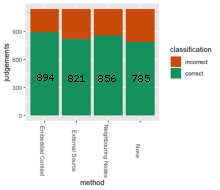
\includegraphics[width=0.75\textwidth]{plots/comparison/barplot_all_judgements}
	 \caption{Combined accuracy of crowdsourcing methods}\label{fig:results_accuracy_combined}
\end{figure}

\paragraph{For which concepts were the crowd wrong?}
Even though the results underlined the usefulness of context for crowds-sourced ontology validation, we were also interested under which circumstances they failed. In particular, we evaluated for which concepts the crowd had most problems with. The goal was to identify common patterns to guide future improvements. 

\hyperref[table:combined_evaluation_bad_concepts]{Table~\ref*{table:combined_evaluation_bad_concepts}} lists 6 concepts that had the highest number of erroneous judgements. The concept \emph{sceptic} is located on the top-most row of the table. None of the judgements were correct for that concept. 
Consequently, for the climate change ontology, the concept was rejected even with context being present. An explanation of that could be the fact
the context was too generic or inappropriate. Clearly, the concept could be associated with climate change, meaning someone who doubts global warming.
Unfortunately, we were not able to adapt context because we had not access to the sources where the ontologies were learned from. 
In most cases though, we expect ontology engineers to have enough knowledge for providing more accurate descriptions that support the crowd.
\begingroup
\renewcommand{\arraystretch}{1.5}
\begin{table}
	\begin{tabularx}{\textwidth}{l c*{4}{Y}}
		\toprule
		\multirow{2}{*}{\emph{Concept}} & \multicolumn{4}{c}{\emph{Methods}} & \emph{Accuracy}\\
		\cmidrule(lr){2-5} \cmidrule(lr){6-6} 
		 & EC & NN & ES & NONE & Total\\
		\midrule
		sceptic & 0/5 & 0/5 & 0/5 & 0/5 & 0/20 \\
		greenhouse & 0/5 & 1/5 & 0/5 & 0/5 & 1/20 \\
		pipeline & 0/5 & 0/5 & 1/5 & 0/5 & 1/20 \\
		consensus & 2/5 & 0/5 & 0/5 & 0/5 & 2/20 \\
		denier & 2/5 & 0/5 & 0/5 & 0/5 & 2/20 \\
		production & 1/5 & 1/5 & 0/5 & 0/5 & 2/20 \\
		\bottomrule
	\end{tabularx}
	\caption{Concepts where most crowd workers had problems~(EC=Embedded Context, NN=Neighbouring Nodes, ES=External Source, NONE=No Context)}
	\label{table:combined_evaluation_bad_concepts}
\end{table}
\endgroup

For the remaining concepts the situation is similar. We identified a common pattern among the descriptions of these concepts: They were either missing, especially for very specific concepts or too generic. The only solution to both problems we see is collaboration between ontology engineers and domain experts to improve context. 

\paragraph{What other observations were found?}
A general phenomenon of all approaches was the relatively high value of precision indicating that the crowd tends to rather reject concepts in case 
of uncertainty or lack of knowledge. However, in ontology engineering recall is often more important than precision. Domain experts and ontology maintainers prefer deleting a few concepts rather than missing some important concepts. 

The second observation was that not all enrichment methods worked best in all scenarios: 


The third observation was that context can be even distracting in rare cases: 